Bevor genauer in die Arbeit eingestiegen werden kann, müssen jedoch erst mal die Ausgangssituation dargestellt, ein paar Begriffe geklärt und das Thema etwas abgesteckt werden.

\section{Projektbeschreibung}
Zu Beginn der Arbeit bestand bereits eine Website, die durch einen internen Workshop konzeptioniert und durch ein Pflichtpraktikum implementiert wurde. Die Website wurde mit der Web-Technologie Elixir gebaut, die sowohl Frontend als auch Backend beinhaltet. Hierbei handelt  es sich um eine Plattform, die das Ziel hat, das Verleihen und Leihen innerhalb von Bekanntschaftskreisen zu vereinfachen/ ermöglichen. Hierfür kann jeder Nutzer seine eigenen, verleihbaren Gegenstände auf der Plattform eintragen. Zusätzlich können Nutzer sogenannte Kreise erstellen und zusammen mit Freunden bzw. Familie beitreten. Jeder kann dann die Gegenstände sehen, die in den verschiedenen Kreisen verfügbar sind, in denen er Mitglied ist. Zur Kontaktaufnahme gibt es ein Chatsystem, bei dem sich Leute Nachrichten hin und her schicken können, um den Austausch zu organisieren.

\section{Funktionsumfang der Beispiel Anwendung}
Grundsätzlich wurde beim Entwurf des Funktionsumfang versucht, die typischen Funktionalitäten von Applikationen abzubilden. Eine Befragung mobiler Anwendungsentwickler durch JetBrains ergab, dass die wichtigsten Funktionen Datenspeicherung, Kommunikation über Netzwerk, Medienanzeige, Status und Navigationsmanagment, Datensynchronisierung, Dateien lesen/schreiben, Sicherheit, Bezahlung, Berechnungen und Machine Learning sind\cite{JetBrains_miscellaneous_2021}. Natürlich sind gerade der letzte Punkt oder die Bezahlung eine sehr Anwendungsfallspezifische Sache, jedoch gibt es einem einen guten Kompass was eine App so grundlegend Abzudecken hat.
Um den Arbeitsaufwand realistisch zu halten und trotzdem aber einige der oben genannten Parameter abzudecken, ist die Implementierung wie im Folgenden beschrieben eingeschränkt:

Allgemein soll eine App gebaut werden, die wie bereits erwähnt sich an einer bestehende Webanwendung orientiert und einen Teil der Funktionalität durch die Programmierung abbilden soll. Des weiteren wird eine GraphQL-Schnittstelle genutzt um die Daten der Webanwendung zu Nutzen. 

\subsection{nativ und Multiplattform v}
Bei der Nativen und der Multi-Plattform Applikation bilden wir den in Abbildung \ref{fig:pageflow} dargestellten Ablauf ab. Dabei sind diese komplett durch in der Applikation implementierten Seiten dargestellt. Diese sind eine Startseite, eine Login- , Profil- , Kommunikations- und einer Chatseite. Dadurch schaffen wir es, die oben genannte Aspekte bis auf Bezahlung und Machine Learning, die für diese Applikation auch kein Anwendungsfall haben, größtenteils abzudecken. Denn durch den Login etwa erfüllt die Applikation teilweise die Bereiche Sicherheit, Statusmanagment, Daten lesen/schreiben und Kommunikation über Netzwerk. 

\begin{figure}[ht]
  \centering
  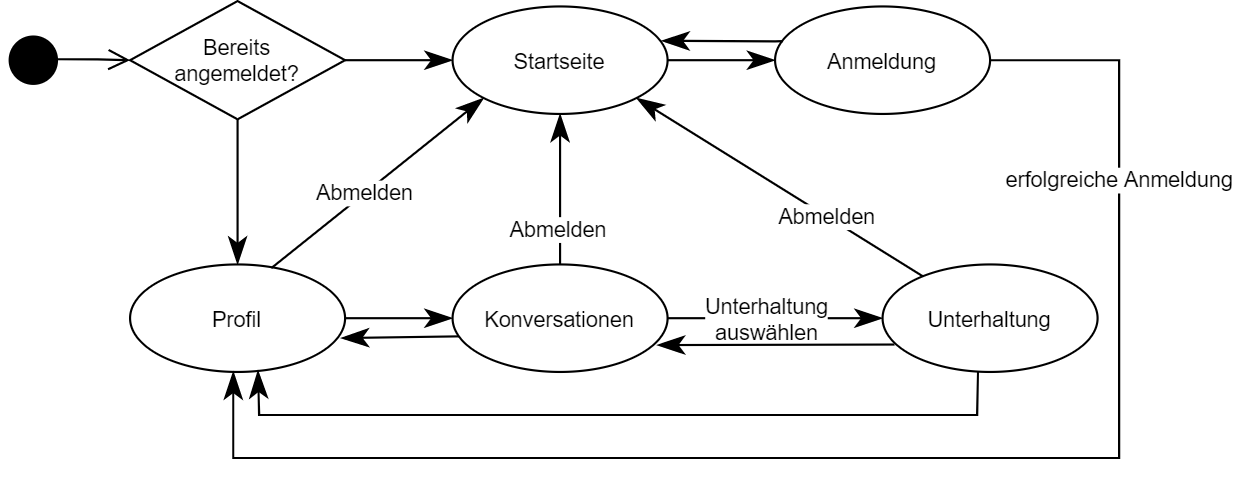
\includegraphics[height=7cm,keepaspectratio]{images/Pageflow_native_flutter.png} 
  \caption{Verbindungen zwischen den Seiten der implementierten Applikation beim nativen Ansatz und dem Multi-Plattform-Ansatz}
  \label{fig:pageflow}
\end{figure}

Der genaue Ablauf der App ist, dass der Nutzer die App öffnet. Ist er beriets eingelogt, wird er automatisch auf die Profil Seite übergeleitet, auf der seine eigenen Sachen angezeigt werden. Ist er nicht angemeldet, so landet er auf einer Startseite/ Willkommensseite, auf der einige Sachen über das Projekt erklärt werden und kann dann zu der Loginseite weiter, von der er nach erfolgreichem Anmelden zu der bereits erwähnten Profilseite kommt. Über einen Knopf in der Menüleiste der App kann der eingeloggte Nutzer auf die Konversationsseite wechseln. Hier wird im eine Liste an Konversationen angezeigt, an denen er beteiligt ist. Nun kann er durch einen Klick auf eine Unterhaltung zu dem Chat wechseln, kann hier die bereits bestehenden Nachrichten lesen und neue Nachrichten abschicken. Mit der Zurück-Taste kann er dann wieder zu der Konversationsseite zurückkehren oder über einen Klick auf das Logo zur Profilseite zurückkehren. Als letztes ist in der Menüleiste noch ein Knopf mit dem Text "Abmelden". Wenn man diesen drückt, werden die gespeicherten Zugangsdaten gelöscht und der Nutzer somit abgemeldet. Nach erfolgreichem Abmelden wird er dann wieder zu der Startseite zurückgeführt.

\subsection{hybrider Ansatz und Mix Ansatz}
Bei den hybriden Absätzen wird die Website mit in die Applikation eingebunden. Je nach Art des hybriden Ansatzes unterscheidet sich hier der Umfang und Ablauf. So wird etwa bei den in Kapitel 4.2 vorgestellten Implementierungen unter Umständen nur die Website in einer Applikation angezeigt. In Kapitel 4.4 jedoch wird die oben erklärte Implementierung mit einer Anzeige der Website gemischt. So wird im vergleich zu Abbildung \ref{fig:pageflow} die Startseite durch die Startseite der Webseite ersetzt. Zusätzlich dazu wird durch eine veränderte Navigation über ein Seitenmenü die zusätzliche durch die Webanwendung verfügbare Funktionalität durch Verlinkung hinzugefügt. Etwa kommen hierdurch eine Übersicht der Kreise in denen der Nutzer Mitglied ist oder eine Liste der Gegenstände die man ausleihen kann hinzu.

\section{Themenabgrenzung}
In der Arbeit werden die Implementierungen auf eine Android Implementierung beschränkt, insofern sie nicht durch das Framework automatisch mitgeliefert werden. Das hat zwei Hauptgründe. Einerseits um den Aufwand für die Implementierung zu beschränken und andererseits sind iOS und Android insofern vergleichbar, da beide nativ auf die vollständigen Funktionalitäten der Betriebssysteme zugreifen. Außerdem sind es nicht die verschiedenen Programmiersprachen und ihre Kleinigkeiten die entscheidend sind, um native Apps zu entwickeln, sondern die Konzepte. So sagen Goadrich et Al in einer Untersuchung, welche Plattform für einen Universitätskurs passend wäre, dass etwa beide Umgebungen fähig sind sowohl 2D als auch 3D Graphiken mit OpenGL und Datenbanken und ihr Managment mit SQLite zu erzeugen.\cite{iOSvsAndroid}Weiter sagten sie, dass Studenten praktische Beispiele von integrierten Betriebssystem sehen könnten und lernen würden mit Threading, Synchronisierung und Locking umzugehen\cite{iOSvsAndroid}. Sie kommen am Ende auf den Schluss, dass es wegen diesem und anderem, kein Unterschied macht welche Plattformumgebung genau gelehrt wird und dass eine Programmierung, mit egal welchem, helfen würde, die Grundideen der mobilen Programmierung zu vermitteln. \cite{iOSvsAndroid}
Natürlich gibt es kleinere und größere Unterschiede zwischen den Programmiersprachen und der Implementierung auf den Plattformen, aber die Nutzung der Betriebssystemspezifischen Schnittstellen und die dahinter liegen Konzepte sind grundlegend gleich.
\TODO{Kein wörtliches Zitat. Übersetzt und nur Sinn mäßig und Ende vervollständigen}

Des weiteren wird in dieser Arbeit eine Möglichkeit der Spieleimplementierung nicht betrachtet. Diese stellen zwar immerhin einen großen Teil der in den Appstores vorhandenen Anwendungen dar, Jedoch sind dies keine typischen Apps die von Appagenturen oder privaten Entwicklern produziert werden, sondern eher von Unternehmen mit Grafikentwicklungs- oder Spieleentwicklungshintergrund. Außerdem werden die meisten Apps nicht in Kotlin oder Swift direkt entwickelt sondern mit Game- und Grafik Engines. Zwar gibt es auch Ansätze, wie Flutter Flame, eine Libary die helfen soll, 2D Games mit Flutter zu entwickeln, 
\TODO{Schlusssatz}
\TODO{Quellen}

\section{Begriffe}
wda
\TODO{Hier noch Sachen umstellen, hinzufügen, und eventuell an Start des Kapitels stellen}
Wenn in dieser Arbeit von einer App oder Applikation geredet wird, so ist hiermit eine Anwendung gemeint, die für mobile Endgeräte, vor allem Smartphones mit den Betriebssystemen Android beziehungsweise iOS gebaut wurden.

Außerdem ist in dieser Arbeit oft die Rede von Multi-Plattform-Anwendungen. Darunter versteht man eine Anwendung, die nicht nur für eine Plattform geschrieben wurde, sondern für mehrere. Dies beinhaltet dann beispielsweise die verschiedenen Smartphone Plattformen, oder aber auch die verschiedenen PC Plattformen wie Linux oder MacOS. Eine Anwendung muss dabei auch nicht alle Plattformen beinhalten, sonder kann auch nur zwei abdecken. Statt Multi-Plattform-Anwendungen wird häufig auch Cross-Plattform-Applikationen als Begriff genutzt, da dies ein in der Industrie häufig benutztes Synonoym ist. 

\section{Die verschiedenen App Development Framework Klassen}
Wenn man über Applikationsentwicklung für mobile Endgeräte spricht, muss man zwischen \TODO{genaue Zahl einfügen} verschiedenen Varianten unterscheiden.
\subsection{Native Applikationen}
Native Apps sind Applikationen die entwickelt werden um auf einer spezifischen Plattform, abhängig des Gerätetyps, des Betriebssystems und der Version zu laufen. Der Quellcode wird dafür zu ausführbaren Code übersetzt.\cite{IEEE_development_classes}
Das bedeutet, dass etwas um eine native Android App zu erstellen, wird diese etwa in Kotlin, die Plattform typische Programmiersprache, programmiert und im Anschluss in Bytecode übersetzt.

Der Vorteil der nativen Entwicklung ist, dass man die Funktionen der verschiedenen Plattform optimal ausnutzen kann. So ist etwa eine Nutzung der Kamera, GPS, Beschleunigungssensoren, Kalender und vielem mehr denkbar einfach. Es gibt eindeutig definierte Schnitstellen und diese müssen nur aufgerufen werden. Dabei ist die Ausführung nicht nur schnell sondern kann auch einfach im Hintergrund ausgeführt werden. Auch eine Benachrichtigung des Nutzers ist problemlos möglich, da man einfach die Schnittstellen der Plattform nutzen kann. Außerdem funktionieren sie, mit eventueller Funktionseinschränkung, auch ohne, dass der Nutzer mit dem Internet verbunden ist. \cite{IEEE_development_classes}

Ein weiterer Vorteil ist, dass man die volle Kontrolle über das Aussehen und der Funktionsweise innerhalb der Plattformgrenzen hat. So kann man dass man vollständig angepasste Nutzeroberflächen bauen, die auf die mobile Plattform aber vor allem an die eigene App angepasst sind. Man ist dadurch nicht abhängig von den Funktionsmöglichkeiten möglicher Zwischenschichten.

Einer der größten Nachteile der nativen Entwicklung jedoch ist der Aufwand und die damit verbundenen Kosten, um für die verschiedenen Plattformen eine Applikation anbieten zu können. Denn die Applikation muss größtenteils für jede Plattform komplett neu gebaut werden. Doch nicht nur die Programmierung ist ein Kostenfaktor. So nennt Delia et Al als weitere Faktoren das Testen, Wartung und Verteilen neuer Version als weitere Faktoren, die auf jeder einzelnen unterstützten Plattform auftreten.\cite{IEEE_development_classes} Dazu kommt, dass man für jede Plattform auch Entwickler benötigt, da sich die wenigsten Entwickler auf allen Plattformen auskennen und Anwendungen für die verschiedenen Plattformen oft auch gleichzeitig entwickelt werden sollen. Dadurch werden aus Anwendungen die auf mehreren Plattformen veröffentlicht werden, schnell große Kostenproduzenten. Deswegen werden hier oft bei kleineren Anwendungen die Implementierung auf eine oder zwei Plattformen beschränkt, was die Reichweite der App vermindert.

\subsection{Web Applikationen}
Web Applikationen sind Applikationen, die einfach nur im Netz verfügbar sind. Sie sind darauf ausgelegt, als Webseiten auf einem Server zu laufen und dann über den Browser der Geräte aufgerufen zu werden. Dieser Ansatz ist denkbar einfach, da bereits einfachste Seite sofort für jeden Nutzer verfügbar sind, sobald sie auf dem Server gestartet wurden. Sie müssen auch nur lediglich einmal entwickelt werden, da sie auf allen Geräten mit einem Browser und einer Internetverbindung aufgerufen werden können. So kann man alle Plattformen mit nur einem Code abdecken.\cite{IEEE_development_classes}

Dennoch hat man hier große Einschränkungen, da sie lediglich die Funktionalitäten zur Verfügung haben, die der Browser anbietet. So können die nativen Schnittstellen nicht genutzt werden und sind in ihrer Funktionalität stark beschränkt. Dazu kommt, dass wenn keine Internetverbindung vorhanden ist, die Anwendung gar nicht genutzt werden kann und bei einer langsamen Internetverbindung die Performance signifikant sinkt. 

Diese Klasse wird jedoch in dieser Arbeit nicht behandelt, da hier auf Anwendungen konzentriert wird, die sich auf einem Gerät installieren lassen und somit als Programme auf dem Gerät verfügbar sind.

\subsection{Hybride Applikationen}
Eine Klasse die dafür durchaus in der Arbeit untersucht wird ist die der hybriden Apps. Diese sind Applikationen die zu einem Teil aus nativem Code besteht und zu einem anderen Teil aus einem Web-Container. Sie benutzen also Web-Technologien, benutzen aber nicht den Browser, sondern einen Web-Container. Unter Umständen kann dieser mit Hilfe von bestimmten API-Schnittstellen auf Gerätespezifische Funktionen zugreifen.\cite{IEEE_development_classes}


\subsection{Cross Plattform Applikationen}
3. Cross-Plattform-Apps
Unterscheidung zwischen Webview in App und z.B. Flutter 
